\documentclass[doc,natbib,12pt]{apa6}

\usepackage[american]{babel}
\usepackage[utf8x]{inputenc}
\usepackage{amsmath}
\usepackage{graphicx}
\usepackage[colorinlistoftodos]{todonotes}
\usepackage{varioref}
\usepackage[hidelinks]{hyperref}
\usepackage[T1]{fontenc}

\title{Memory Management}
\shorttitle{Memory Management}
\author{Youwei Lu}
\affiliation{CISC 530-51- A-2018/Late Fall Assignment 1}

%\abstract{Referring to Operating Systems architecture, the topic of this assignment is on the ``Memory Management'' which is part of the computer's physical memory or Random-Access Memory (RAM) organization.}

\begin{document}
	\maketitle
	
	\section{Introduction}
	
	Memory management is a kind of resource management about the memory use in computer. Memory management is a crucial part of both programming and system administration. To dynamically allocate portions of memory for programs, and find a way to reuse it when no longer needed. This is very important to any computer systems as more than a single process is running at a time. \citep{Gibson1988}
	
	Most of the time, a program is a binary executable file. The application must be in memory for execution. The process must be moved between disk and memory back and forth during execution.
	
	The object of memory management is like this: this function keeps records of the status of each memory address, either allocated or free. It determines when to allocate, get, use, how much the memory a program uses. As the memory is there, the function also determines the location, and update the status of address. \citep{Madnick1974}
	
	Before any management can be discussed, we need to understand the basic concept, memory address, thus at the beginning of this study, a memory address is introduced. The address space in the whole memory of a process is studied on page~\pageref{chp:processAddressSpace}, and three address express methods (symbolic, relative, and physical addresses)  are following on page~\pageref{chp:symbolicAddress}, page~\pageref{chp:relativeAddress} and page~\pageref{chp:physicalAddress}. Then we studied several memory management techniques. Developers have the abilities to choose from static and dynamic loading at the time of writing programs (on page~\pageref{chp:staticDynamicLoading} ), and of course the corresponding `linking' concept is discussed on page~\pageref{chp:staticDynamicLinking}. Next, we will discuss the techniques used in an operating system. One basic concept is `swapping' for storing process between main and secondary memories (on page~\pageref{chp:swapping}). For the memory of a certain program, memory allocation is introduced on page~\pageref{chp:memoryAllocation}, followed with detail discussion of the two ways of allocation: single-partition allocation (on page~\pageref{chp:singlePartitionAllocation}) and another one is multiple-partition allocation (on page~\pageref{chp:MultiplePartitionAllocation}). Along with partition allocation, one must consider the possible fragmentation (on page~\pageref{chp:fragmentation}), and this concept can be divided into two parts for detail discussing: external fragmentation (on page~\pageref{chp:externalFragmentation}) and internal fragmentation (on page~\pageref{chp:internalFragmentation}). The following of this study then focuses on the way of dividing the memory into basic units, paging (on page~\pageref{chp:paging}) and segmentation (on page~\pageref{chp:segmentation}), and comparing them. The way of paging or segmentation works between a logical address, and a physical address is introduced in address translation on page~\pageref{chp:addressTranslation}.
	
	As a summary and page reference, complete explanation is given for the following issues:
	
	\begin{itemize}
		\item Process Address Space (page~\pageref{chp:processAddressSpace})
		
		\item Types of Addresses (page~\pageref{chp:typesAddresses})
		
		\item Symbolic addresses (page~\pageref{chp:symbolicAddress})
		
		\item Relative addresses (page~\pageref{chp:relativeAddress})
		
		\item  Physical addresses (page~\pageref{chp:physicalAddress})
		
		\item  Static vs Dynamic Loading (page~\pageref{chp:staticDynamicLoading})
		
		\item  Static vs Dynamic Linking (page~\pageref{chp:staticDynamicLinking})
		
		\item Swapping (page~\pageref{chp:swapping})
		
		\item  Memory Allocation (page~\pageref{chp:memoryAllocation})
		
		\item   Single-partition allocation (page~\pageref{chp:singlePartitionAllocation})
		
		\item   Multiple-partition allocation (page~\pageref{chp:MultiplePartitionAllocation})
		
		\item  Fragmentation (page~\pageref{chp:fragmentation})
		
		\item   External fragmentation (page~\pageref{chp:externalFragmentation})
		
		\item   Internal fragmentation (page~\pageref{chp:internalFragmentation})
		
		\item  Paging (page~\pageref{chp:paging})
		
		\item  Address Translation (page~\pageref{chp:addressTranslation})
		
		\item  Segmentation (page~\pageref{chp:segmentation})
		
	\end{itemize}
	
	
	
	
	
	
	
	
	
	\newpage
	\section{Process Address Space} \label{chp:processAddressSpace}
	
	A process is defined as an instance of a program running. We can treat it as a task, which is also a word used in many operating systems. We start a process when initiating a program, either by a shell command or from the user, GUI operating, or from another application. A particular collection of data is related to the process so that the process can be tracked. 
	
	Address space is all the memory a process a allocate, usually large memory. Each process running has its own virtual address space, usually 4GB block in a 32-bit mode. The virtual addresses also can be mapped to physical memory, by the way of page tables, and each process own one page table. In a word, we have seen an essential property of process address space: a process and an address space is 1:1 mapping.
	
	Another critical factor about address space is that the address space is in a protected domain. The operating system isolates address spaces that one process can't even see another address. The same pointer address is used in different processes point to different memory. Also note that after enabling the virtual address, it is used by all software in the machine, including the kernel. It's also possible that while the process is running, the process space can change mapping dynamically.
	
	\begin{figure}[h]
		\centering
		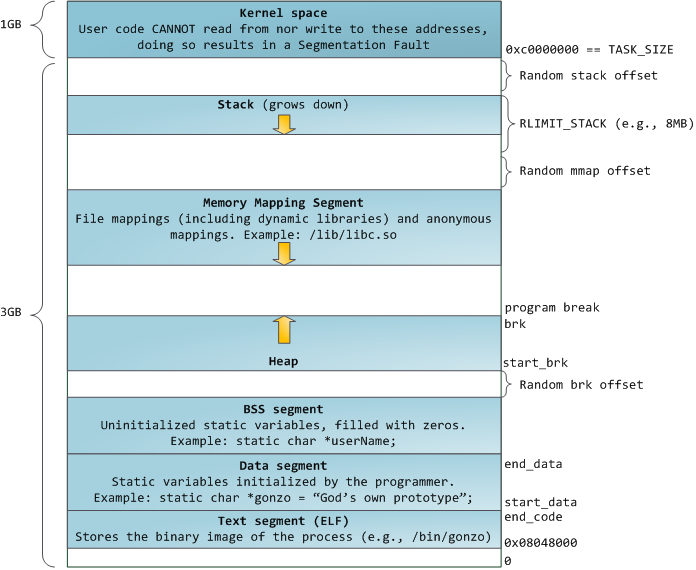
\includegraphics[width=1\textwidth]{linuxFlexibleAddressSpaceLayout.png}
		\caption{\label{fig:memoryLayout}A typical memory layout. \citep{Duarte2009}}
	\end{figure}
	
	Figure~\vref{fig:memoryLayout} shows a typical memory layout in a Linux system. Note that the starting virtual address was the same for all process in a machine. This could be vulnerable to security. Therefore, address space randomization is popular, often applied after space initialization. With that in mind, let's take a closer look at each segment:
	
	\subsection{Kernel space}
	After enabling the virtual address, it is used by all software in the machine, including the kernel itself, so kernel always keep a portion of the virtual address space. However, the kernel doesn't need that much, instead, it only needs the portion to map the physical memory it needs. In many operating systems, the same physical memory is used in all processes' kernel space. Kernel code and data should always be addressable and can handle interruptions or systems calls.
	
	\subsection{Stack}
	The program stack is contained in the stack area. As we know, stack has a LIFO(Last In First Out) structure. At a x86 computer the stack area increases toward to the address 0, while it may go to opposite direction on some other architectures. A register tack (pointer) tracks the stack and is changed every time a value enters into the stack. This set of values pushed is called a ``stack frame'', and should contain at least a return address.
	
	Automatic variables and information saved by the function are stored in the stack. When the system calls a function, the information about the address to return to and the environment are saved in the stack. For a recursive function call, a new stack is used. Thus, the variables are not shared in different recursive operations.
	
	\subsection{Memory mapping segment}
	Below the stack, we have the memory mapping segment. Here the kernel maps contents of files directly to memory. Memory mapping is a convenient and high-performance way to do file I/O, so it is used for dynamic loading libraries. It is also possible to create an anonymous memory mapping that does not correspond to any files, being used instead for program data. It is possible to request a large amount of memory by creating an anonymous mapping.
	
	\subsection{Heap}
	We usually have dynamic memory allocation resides in heap segment. The heap area has very large address from the end of BSS segment. Shared libraries will share the heap area.
	
	\subsection{BSS segment} 
	The BSS segment is named after an assembler operator well known as ``block started by symbol'' \citep{Stevens1992}. Nowadays, this segment is usually called ``Uninitialized data segment''. Kernel initialized this segment to arithmetic 0 before any program starts executing. Every public data, including global variables and static variables, are initialized to zero, a common example is the variables declared in for-loop.
	
	\subsection{Data segment}
	The Data Segment is also called as Initialized Data segment. This is part of program's virtual address space, containing global variables and static variables initialized. This segment is also commonly separated into read-only area and read-write area.
	
	\subsection{Text segment}
	The text segment is also called as a code segment. It is the section containing executable instructions. Most of the time, we make the text segment read-only, as a program may accidentally modifying its instructions.
	
	\newpage
	\section{Types of Addresses} \label{chp:typesAddresses}
	For the logical addresses of a process, the mapping of logical address to physical address is allocated by the operating system. There are in total three types of addresses before after memory allocation \citep{Silberschatz2001}:
	
	\begin{itemize}
		\item Symbolic addresses: The address for source code. It contains the variable names and constants.
		\item Relative addresses: The address at the time of compilation, and symbolic address are converted into relative addresses.
		\item Physical addresses: The address generated by the loader when a program enters main memory.
	\end{itemize}
	
	Details of the three types of addresses will be given in the following sections, on page~\pageref{chp:symbolicAddress}, page~\pageref{chp:relativeAddress} and page~\pageref{chp:physicalAddress}.
	
	\newpage
	\section{Symbolic Addresses} \label{chp:symbolicAddress}
	
	Before symbolic addresses, we need to know what an absolute address is, which is simply an identifier and a memory location, for example, 0x0012. However, this address is complicated for a developer to remember and identify.
	
	A symbolic address is a kind of scheme that the reference to an address is made by some convenient symbol \citep{Oxford2004}. Of course, we are choosing some symbols. The programmer writes the symbols in the code, and some kind of computable address replaces the symbolic address during compiling by an assembler.
	
	How does it work? Our source code produces symbolic addresses, it could be a variable a programmer write or an abstraction offered to us by our assembler. Then a compiler will bind these symbolic address into two parts: absolute addresses and relocatable address. For the relocatable address, loader makes the final binding without dynamic relocation.
	
	Table~\vref{tab:symbolicAddress} shows an example of binding the symbolic address `x'. We can clearly see that symbolic address is much more easier to be read than absolute address.
	
	\begin{table}[h]
		\centering
		\begin{tabular}{l|r}
			Item & Address \\\hline
			Symbolic Address & x \\
			Absolute Address & 0x04  \\
			Relocatable address & 16 bytes from the beginning of the file
		\end{tabular}
		\caption{\label{tab:symbolicAddress}An example of symbolic address binding.}
	\end{table}
	
	\newpage
	\section{Relative Addresses} \label{chp:relativeAddress}
	The relative address is a concept comparing to an absolute address. An absolute address is a location defined by developer. However, for coding convenience, we usually need to use the relative address that has some distance from a certain point as a base address. The absolute address of that memory is calculated by adding it to the base address.
	
	Figure \ref{fig:relativeAddress} gives an example of relative address. The memory address 5 can be represented as B+4, and its absolute address is 5 only if the base address is 1.
	
	\begin{figure}[h]
		\centering
		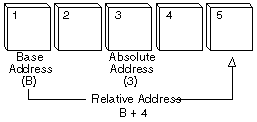
\includegraphics{relative-address.png}
		\caption{\label{fig:relativeAddress}An example of absolute and relative addresses. \citep{Beal2018}}
	\end{figure}
	
	\newpage
	\section{Physical Addresses} \label{chp:physicalAddress}
	Unlink virtual memory, physical address is just  the basic binary number (0 and 1) presenting logical high and low states, in and address bus. The primary storage or I/O device has a cell that corresponds the bus.
	
	Memory management is used in a computer with virtual memory, since physical address and virtual address are different. Virtual address needs to be mapped into physical address. Therefore, the running application can visit the whole primary memory with easily readable virtual addresses.
	
	\newpage
	\section{Static vs Dynamic Loading} \label{chp:staticDynamicLoading}
	It is the developer's choice to how to load their module dependencies and data by developing programs. while choosing to load program statically, the whole program is complied and linked with all external libraries and dependencies. The linker combines every object program along with other modules and libraries into a single program, including the addresses. Everything is in memory for execution. The dynamic loading, on the other hand, at the time of compilation, the compiler will not compile all libraries or modules, but only provide the references, and the linking work will be done at the time of execution. 
	
	As a summary, static loading loads every module dependencies and data into memory at the time of compilation, while dynamic loading only loads a necessary program, and loads dependencies at the time of execution. It is straightforward to conclude that static loading loads faster, with much larger memory, and more stable; while dynamic loading loads more quickly, with smaller memory needed, but may interrupt programming running while loading dependencies. And this is shown in Table~\vref{tab:staticDynamicLoading}.
	
	\begin{table}[h]
		\centering
		\begin{tabular}{l|rr}
			Loading method & Static & Dynamic \\\hline
			Load time & Slower  & Faster\\
			Memory use & Large & Small  \\
			Runtime & More stable & Less stable
		\end{tabular}
		\caption{\label{tab:staticDynamicLoading}Comparison of Static vs Dynamic Loading.}
	\end{table}
	
	how to choose the way of loading, or balancing of loading is always a hot research topic. Balancing static load is usually based on the behavior information of system; transfer decisions are not considered. However, dynamic polices should consider the transfer decisions as it is relevant to current system state. Therefore, the dynamic polices are more complicate than static ones, and standard optimal policies are only available for several special systems, whereas the balancing in distributed computer systems is studied by \cite{Kameda2000}. They studied the performance between static load and dynamic load in a distributed system. The system has been characterized for both dynamic and static polices. Their study shows that the dynamic policy is better than static one in the average response time, at most 30 percent for the parameter values.
	
	\newpage
	\section{Static vs Dynamic Linking} \label{chp:staticDynamicLinking}
	As explained on the section of Static and Dynamic loading on page \pageref{chp:staticDynamicLoading}, linking is simply the method chosen at the time of static loading or dynamic loading. At the situation of static loading, static linker combines all modules needed into a single one, and doesn't need any at runtime. While in the case of dynamic loading, the dynamic linker saves much less but only the dependencies needed to start, and everything else is referenced.
	
	\newpage
	\section{Swapping} \label{chp:swapping}
	To discuss swapping, we must first understand that a process needs to be in memory, and when memory is limit, a process might be swapped occasionally between a backing memory and the main memory. A backing disk is usually used for storing the memory contents temporarily. This memory reclamation method is called swapping, or memory swapping.
	
	Take a multiprogramming environment as an example. A quantum needs to be swapped out the space after expiring. 
	
		Figure~\vref{fig:swapping} shows an example of swapping, where clearly shows that Process P1 is swapped out to leave space in main memory for Process P3. After the process of Process P3, P3 is swapped out, and Process P1 is taken back to main memory.
	
	Should you use the swapping or not depending on the swapping time. If the swapping takes too much time than the execution time, the swapping might be unnecessary.
	
	\begin{figure}[th]
		\centering
		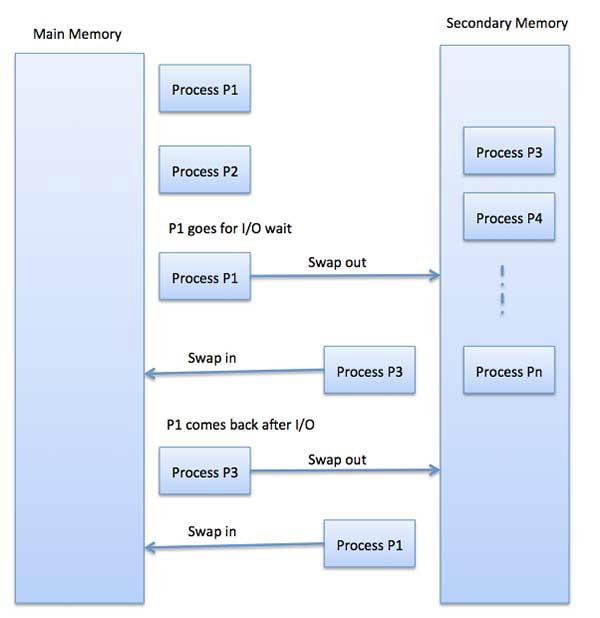
\includegraphics[width=0.8\textwidth]{swapping.png}
		\caption{\label{fig:swapping}Memory swapping demonstration. \citep{tutorialspoint2018}}
	\end{figure}
	
	Assuming the user process is 4096KB, and the data transfer takes about 1MB per second. Then the transfer of 1024K process from to memory takes
	\begin{verbatim}
	4096KB / 1024KB per second
	= 4 seconds
	= 4000 milliseconds
	\end{verbatim}
	For both out and in time, the transfer take 8000 milliseconds, and plus other overhead.
	
	\newpage
	\section{Memory Allocation} \label{chp:memoryAllocation}
	Memory allocation is the process of setting aside sections of memory in a program to be used to store variables, and instances of structures and classes. It is usually a computer hardware operation but is managed through operating system and software applications. The concept of memory allocation is quite similar in physical and virtual memory management. Programs are assigned with a specific memory per requirement at the time of executing. Once the program has finished its operation or is idle, memory is released and allocated to another program or merged within the primary memory.
	
	Main memory usually has two partitions:
	\begin{itemize}
		\item Low memory - Operating system resides in this memory.
		\item High memory - User processes then held in high memory.
	\end{itemize}
	
	To fully benefit from both the low and high memories, the operating system uses the following two different memory allocation mechanisms: Single-partition allocation and Multiple-partition allocation.
	
	In Single-partition allocation, the relocation-register scheme is used to protect user processes from each other, and from changing operating system code and data. Relocation register contains a value of smallest physical address whereas limit register contains the range of logical addresses. Each valid address must be less than the limit register.
	
	In Multiple-partition allocation, main memory is divided into many fixed-sized partitions where each partition should contain only one process. 
	When a partition is free, a process is selected from the input queue and is loaded into the free partition. When the process terminates, the separation becomes available for another operation.
	
	In the following sections on page \pageref{chp:singlePartitionAllocation} and \pageref{chp:MultiplePartitionAllocation}, both partition mechanisms will be discussed separately.
	
	\newpage
	\section{Single-partition Allocation} \label{chp:singlePartitionAllocation}
	In the case of allocating all memory in a single partition, the operating system is residing in low memory, and the user processes are executing in high memory. 
	
	The operating system code and data should be protected from changes by the user processes, and we still need to protect the user processes from one another. We can provide both protections by using a relocation register.
	
	The relocation register contains the value of the smallest physical address, and the limit register contains the range of logical addresses. With the relocation and limit registers, each logical address must be less than the limit register. Then the Memory Management Unit (MMU) is responsible for mapping the logical address dynamically by adding the value in the relocation register. This mapped address is finally sent to memory. The process is shown in Figure~\vref{fig:singlePageAllocation}. We can clearly see that the address from CPU is passing the limit register and relocation register, and then mapped as the physical address into RAM.
	
	\begin{figure}[h]
		\centering
		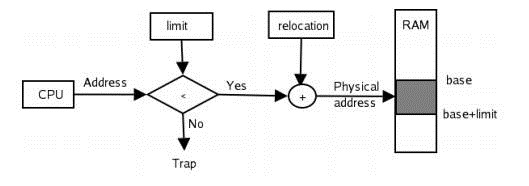
\includegraphics[width=1\textwidth]{singlePageAllocation.jpg}
		\caption{\label{fig:singlePageAllocation}Hardware support for relocation and limit registers. \citep{Vissicomp2014}}
	\end{figure}
	
	The relocation-register scheme provides an effective way to allow the operating-system size to change dynamically.
	
	\newpage
	\section{Multiple-partition Allocation} \label{chp:MultiplePartitionAllocation}
	Another simple way to deal with memory allocation is to divide memory into a number of fixed-sized partitions. Each partition may contain exactly one process.
	
	Thus the degree of multiprogramming is bound of partitions. When a partition is free, a process is selected from the input queue and is loaded into the free partition. When the process terminates, the partition becomes available for another operation.
	
	The operating system keeps a table indicating which parts of memory are available and which are occupied.
	
	Initially, all memory is available for user processes and is considered as one large block, of available memory, a hole. When a process arrives and needs memory, the operating system forms a hole large enough for this process.
	
	When a process arrives and needs memory, we search this set for a hole that is large enough for this process. If the hole is too large, it is split into two: One part is allocated to the arriving process; the other is returned to the set of holes. When a process terminates, it releases its block of memory, which is then placed back in the collection of holes. If the new hole is adjacent to other holes, we merge these adjacent holes to form one more massive hole.
	
	Figure~\vref{fig:multiplePartitionAllocation} shows an example of the holes of the memory partition. Initially, Process 2, process 8 and process 5 occupy all memory. After process 8 terminated, it's memory partition is available for other operations. Then process 9 uses part of the `hole', while there's another free `hole' for other processes, which continues to be separated, for process 10, and a smaller free `hole'.
	
	\begin{figure}[h]
		\centering
		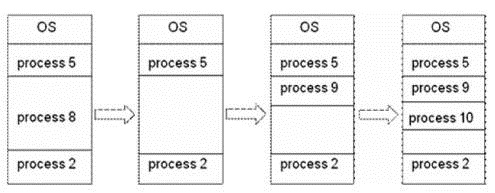
\includegraphics[width=1\textwidth]{multiplePartitionAllocation.jpg}
		\caption{\label{fig:multiplePartitionAllocation}Example of multiple partition allocation. \citep{Vissicomp2014}}
	\end{figure}
	
	This procedure is a particular instance of the general dynamic storage-allocation problem, which is how to satisfy a request of size n from a list of free holes. There are many solutions to this problem \citep{Petzold2000}:
	
	\begin{itemize}
		\item First-fit: Find the first hole where the waiting program will fit. Allocate the first hole that is big enough. Searching can start either at the beginning of the set of holes or where the previous first-fit search ended. We can stop searching as soon as we find a free hole that is large enough. This is a fast algorithm but usually leaves a smaller hole, except where the fit is an exact size.
		\item Best-fit: Find the hole that best fits the job. i.e., with the least left over. Allocate the smallest hole that is big enough. We must search the entire list unless the list is kept ordered by size. This strategy produces the smallest extra hole.
		\item Worst-fit: Find the biggest hole, leaving the biggest remainder. We must search the entire list unless it is sorted by size. This strategy produces the largest leftover hole which may be more useful than the smaller leftover hole from a best-fit approach. This is usually the partition allocation algorithm chosen by system designers.
	\end{itemize}
	
	
	\newpage
	\section{Fragmentation} \label{chp:fragmentation}
	Continue with the discussion of partition allocation, we know that when a process exits, merging can be done if there is an existing hole above and/or below it. However, we also know that no matter which method we choose in allocation (first-fit, best-fit, or worst-fit), memory leftover I snot avoidable, the only difference is the size. All the useless little holes are described as fragmentation.
	
	It happens after sometimes that processes cannot be
	allocated to memory blocks considering their small size and memory blocks
	remain unused. 
	
	
	The system may get to a point when the available memory is enough to start a process, but it is in the form of holes too small to load the process. As the useless holes are outside of any process' memory, this situation is known as external fragmentation. This can be solved by compaction, by moving existing operations (and their partition registers) to consolidate the holes. The operating system should use an algorithm to minimize the amount of copying to make the compaction as fast as possible.
	
	Figure~\vref{fig:compaction} shows how fragmentation can cause waste of memory
	and a compaction technique can be used to create more free memory out of
	fragmented memory.
	
	\begin{figure}[h]
		\centering
		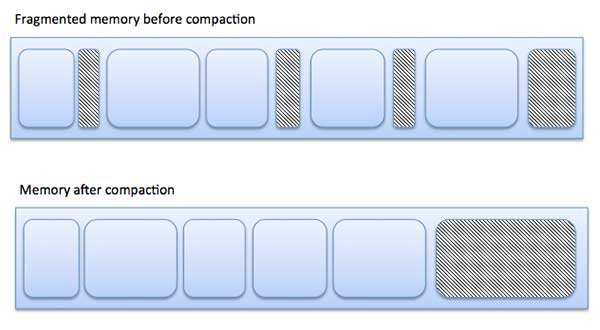
\includegraphics[width=1\textwidth]{compaction.png}
		\caption{\label{fig:compaction}Fragmented memory before and after compaction. \citep{tutorialspoint2018}}
	\end{figure}
	
	There are two different but related forms of fragmentation: external fragmentation and internal fragmentation, which can be present in isolation or conjunction. 
	\begin{itemize}
		\item External fragmentation: Total memory space is enough to satisfy a request or to reside a process in it, but it is not contiguous, and it cannot be used.
		\item Internal fragmentation: We assign a bigger memory block to process. Some portion of memory is left unused, as it cannot be used by another process.
	\end{itemize}
	
	External fragmentation is discussed on page \pageref{chp:externalFragmentation}, and internal fragmentation is discussed on page \pageref{chp:internalFragmentation}.
	
	\newpage
	\section{External Fragmentation} \label{chp:externalFragmentation}
	External fragmentation happens when free memory is separated into small blocks and is interspersed by allocated memory. It is a drawback of certain storage allocation algorithms when they fail to order memory used by programs efficiently. As a result of external fragmentation, although free storage is available, it is not usable because it is divided into pieces that are too small individually to satisfy the demands of the program. The term ``external'' refers to the fact the unusable storage is outside the allocated regions.
	
	For example, consider a situation wherein a program allocates 3 contiguous blocks of memory and then frees the middle block. The memory allocator can use this free block of memory for future allocations. However, it cannot use this block if the memory to be allocated is larger in size than this free block. This example is shown in row 2 in Table~\vref{tab:externalFragmentation}, in which block B is moved. Although there are 4 blocks left, new application bigger than 3 blocks cannot start.
	
	\begin{table}[h]
		\centering
		\begin{tabular}{c|c|c|c|c|c|l}
			\multicolumn{6}{c|}{Blocks} & Comments \\\hline
			A & B  & C & & & & Allocated three blocks A, B, and C\\\hline
			A &     & C & & & & Freed block B. \\\hline
			A & B & & & & & Move C to the position of B. \\\hline
		\end{tabular}
		\caption{\label{tab:externalFragmentation}Example of external fragmentation.}
	\end{table}
	
	
	External fragmentation also occurs in file systems as many files of different sizes are created, change volume, and are deleted. The effect is even worse if a file which is divided into many small pieces is removed because this leaves similarly small regions of free spaces. 
	
	External fragmentation can be reduced by compaction or shuffle memory
	contents to place all free memory together in one large block. For example, Look at Table~\vref{tab:externalFragmentation} again, we can make larger memory available after block C by moving it to the original position of block B, and now any application smaller than 4 can start. Relocation usually is dynamic, as if we want to make compaction.
	
	\newpage
	\section{Internal Fragmentation} \label{chp:internalFragmentation}
	Due to the rules governing memory allocation, more computer memory is sometimes allocated than is needed. For example, memory can only be provided to programs in chunks divisible by 4, 8 or 16, and as a result, if a program requests perhaps 29 bytes, it will actually get a chunk of 32 bytes. When this happens, the excess memory goes to waste. In this scenario, the unusable memory is contained within an allocated region. This arrangement, termed fixed partitions, suffers from inefficient memory use - any process, no matter how small, occupies an entire partition. This waste is called internal fragmentation \citep{Symantec2010}.
	
	Unlike other types of fragmentation, internal fragmentation is difficult to reclaim; usually, the best way to remove it is with a design change. For example, in dynamic memory allocation, memory pools drastically cut internal fragmentation by spreading the space overhead over a more significant number of objects. When designing, try to reduce the internal fragmentation by effectively assigning the smallest partition but large enough for the process.
	
	\newpage
	\section{Paging} \label{chp:paging}
	Paging is a memory management scheme by which a computer stores and retrieves data from secondary storage for use in main memory \citep{Arpaci-Dusseau2014}. In this scheme, the operating system retrieves data from secondary storage in same-size blocks called pages. Paging is an important part of virtual memory implementations in modern operating systems, using secondary storage to let programs exceed the size of available physical memory.
	
	A computer can address more memory than the amount physically installed on
	the system. This extra memory is actually called virtual memory, and it is a
	section of a hard that's set up to emulate the computer's RAM. Paging
	technique plays a vital role in implementing virtual memory.
	Paging is a memory management technique in which process address space is
	broken into blocks of the same size called pages (size is the power of 2, between 512 bytes and 8192 bytes). The size of the process is measured in the number
	of pages.
	
	\begin{figure}[h]
		\centering
		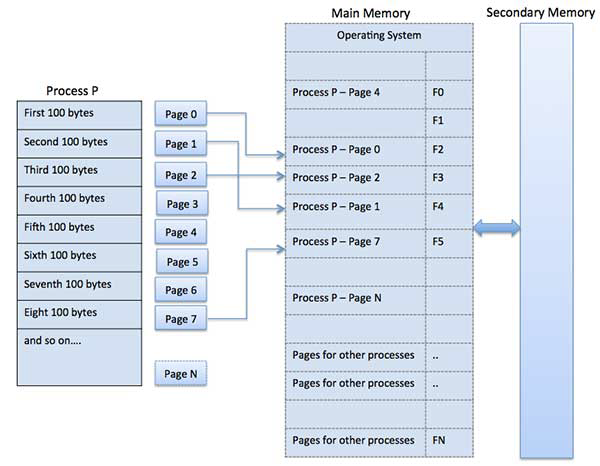
\includegraphics[width=1\textwidth]{paging.png}
		\caption{\label{fig:paging}Pages mapping. \citep{tutorialspoint2018}}
	\end{figure}
	
	Similarly, main memory is divided into small fixed-sized blocks of (physical)
	Memory called frames, and the size of a frame is kept the same as that of a
	page to have optimum utilization of the main memory and to avoid external
	fragmentation. Figure~\vref{fig:paging} shows the paging process. Process P is divided into N pages, each one contains 100 bytes, same sizes. The main memory can put these pages into secondary memory, and load them back for execution.
	
	Paging is designed to reduce external fragmentation, and here is a list of advantages and disadvantages of paging:
	\begin{itemize}
		\item Paging reduces external fragmentation but still, suffer from internal fragmentation.
		\item Paging is simple to implement and assumed as an efficient memory management technique.
		\item Due to equal size of the pages and frames, swapping becomes very easy.
		\item Page table requires extra memory space, so may not be good for a
		system having small RAM.
	\end{itemize}
	
	
	\newpage
	\section{Address Translation} \label{chp:addressTranslation}
	To better understand how pages work in the operating system, we should also be familiar with another term: `frame'. The physical address space is conceptually divided into many fixed-size blocks, called frames. The logical address space is also divided into fixed-size blocks, called pages. Each one is represented by its number and the offset.
	
	\begin{verbatim}
	Logical Address = Page number + page offset
	Physical Address = Frame number + page offset
	\end{verbatim}
	
	Also, note that page size is always equal to the frame size to reduce internal fragmentation.
	
	Now let us consider an example:
	
	\begin{itemize}
		\item Physical Address = 12 bits, then physical address space = 4 K words
		\item Logical Address = 13 bits, then logical address space = 8 K words
		\item Page size = frame size = 1 K words
	\end{itemize}
	
	As can be seen from Figure~\vref{fig:pagingFrame}, we get $2^2$ frames in physical address space and $2^3$ pages in logical address space.
	
	\begin{figure}[h]
		\centering
		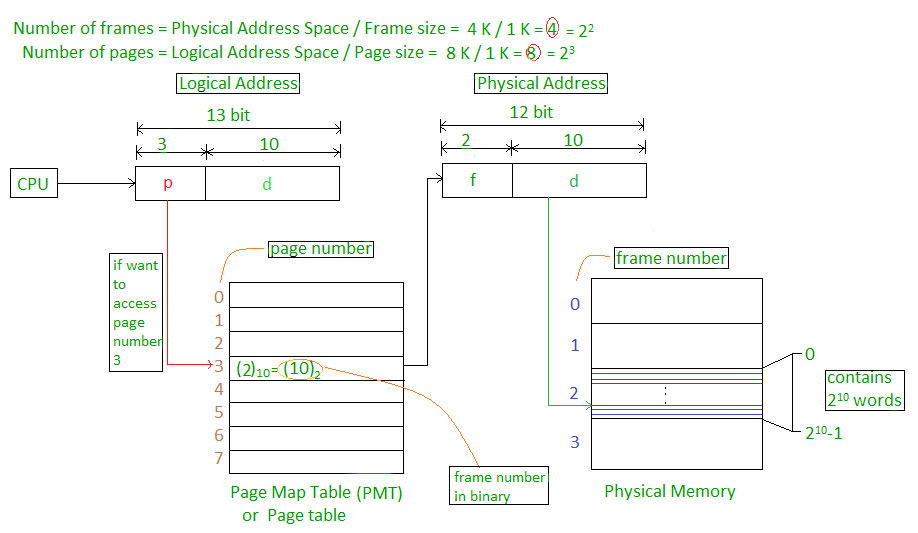
\includegraphics[width=1\textwidth]{pagingFrame.jpg}
		\caption{\label{fig:pagingFrame}Pages mapping. \citep{GeeksforGeeks2018}}
	\end{figure}
	
	In Figure~\vref{fig:pagingFrame},    in the logical address, `p' indicates the page number, which is the number of bits required to represent the pages in logical address space of page number. `d' indicates the page offset, which is the number of bits required to represent a particular word in a page or page size of logical address space or word number of a page or page offset. Similarly, in physical address, `f' indicates the frame number, which is the number of bits required to represent the frame of physical address space or frame number. Also, `d' indicates the frame offset, which is the number of bits required to represent a particular word in a frame or frame size of physical address space or word number of a frame or frame offset.
	
	A data structure called page map table is used to keep track of the relation between a page of a process to a frame in physical memory. When the system allocates a frame to any page, it translates this logical
	address into a physical address and create an entry into the page table to be
	used throughout the execution of the program.
	
	However, if page table contains a large number of entries, then we can use Translation look-aside buffer (TLB), a hardware cache. It is a high-speed cache, and each entry in TLB consists of two parts: a tag and a value. All item is compared with all tags simultaneously, and if the item is found, the corresponding value is returned, as shown in Figure~\vref{fig:TLB}.
	
	\begin{figure}[h]
		\centering
		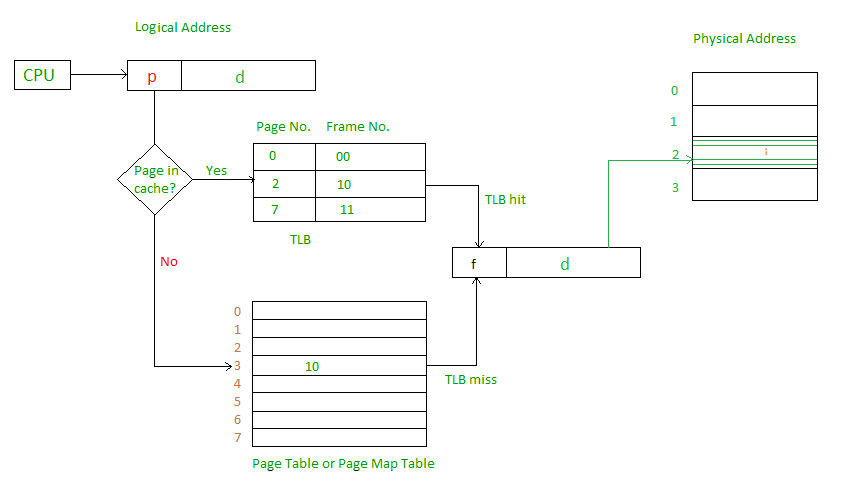
\includegraphics[width=1\textwidth]{TLB.jpg}
		\caption{\label{fig:TLB}Translation look-aside buffer. \citep{GeeksforGeeks2018}}
	\end{figure}
	
	
	\newpage
	\section{Segmentation} \label{chp:segmentation}
	To overcome the shortage of paging, one may consider segmentation. Segmentation is a memory management technique where all job can be divided into several segments of different sizes, one for each module that performs related functions. One segment has a certain logical address of the program. The corresponding segmentation is loaded into non-contiguous memory when a process is executed, while every segment is loaded into a contiguous block of available memory.
	
	Segmentation is very similar to paging, and the only difference is the size: that segments are of variable-length and paging pages sizes are fixed. A program segment may contain the program's primary function, utility functions, data structure, etc. The operating system stores a segment map table for every process and a list of free memory blocks along with segment numbers, their size and memory locations in main memory. For each segment, the table stores the starting address and the length of the part. Same like paging, each segment needs a reference to a memory location that includes a value of identification and offset for the segment. Segments or sections are also used in object files of compiled programs when they are linked together into a program image and when the image is loaded into memory.
	
	Segments usually correspond to natural divisions of a program such as individual routines or data tables, so segmentation is generally more visible to the programmer than paging alone. Different segments may be created for different program modules, or for different classes of memory usage such as code and data segments. Individual segments may be shared between programs. \citep{Englander2003}
	
	In a segment system, we often use a hardware memory management unit (MMU) for translating the segment and offset into a physical address, and also we need to check the translation that the reference and offset is permitted. Each segment has a length and set of permissions (for example, read, write, execute) associated with it. Only the agreements of the segment are allowed by a process to make, and just if the offset within the segment is within the range specified by the length of the segment. Otherwise, a hardware exception is raised.
	
	Segments may also work like paging in virtual memory. In this case, a segment is flagged indicating whether it is in main memory or not. An exception is raised, and the operating system will read the segment into memory from secondary storage if a segment is not present in main memory.
	
	Both segmentation and paging are used for implementing memory protection, and they can be combined. Now let's look at the implementation. Segmentation has been implemented in several different ways on different hardware, with or without paging. Intel x86 memory segmentation does not fit either model and is discussed separately below. \citep{Intel2012}
	
	\subsection{Segmentation without paging}
	When there is no paging involved, each segment is with information that where the segment is located in memory -- the segment base. As a memory location is referenced, we add the offset to segment base to make a physical memory address.
	
	An implementation of virtual memory on a system using segmentation without paging requires that entire segments be swapped back and forth between main memory and secondary storage. When a segment is traded in, the operating system has to allocate enough contiguous free memory to hold the entire segment. Memory fragmentation is possible if there is not enough contiguous memory even if there is enough in total.
	
	\subsection{Segmentation with paging}
	Instead of remembering an actual memory location, with paging, the segment information includes the address of a page table for the segment. When a program references a memory location, the offset is translated to a memory address using the page table. A segment can be extended simply by allocating another memory page and adding it to the segment's page table.
	
	Implementation of virtual memory on a system using segmentation with paging usually only moves individual pages back and forth between main memory and secondary storage, similar to a paged non-segmented system. Pages of the segment can be located anywhere in main memory and need not be contiguous. This reduces memory fragmentation, but the drawback is the reduced amount of input/output between primary and secondary storage.
	
	\newpage
	\section{Conclusion}
	Basic concepts and techniques related to memory management are discussed in this study.
	
	To fully understand memory management, the first concept should be the process address space, and typical memory layout is displayed in this study, including the Kernel space, Stack, Memory mapping segment, Heap, BSS segment, Data segment, and Text segment. Following that, basic memory addresses concept is introduced, and there are three types of addresses used in a program before, and after a memory is allocated, they are Symbolic addresses, Relative addresses, and Physical addresses.
	
	Then we turn our interest into some memory management techniques. For a developer, one can decide the loading method of memory at the time of writing program codes. One can choose static or dynamic loading method, determine among loading time, memory use, or runtime. The corresponding static or dynamic linking is also discussed after it. The next technique discussed is an operating system. Swapping is a primary method to store process memories between main memory and secondary memory, and it is used in a few systems, as the swapping time takes too much-comparing execution time.  As a method to utilize the main memory, memory allocation is then discussed. We should optimize the use between the low memory and high memory, which leads to two methods: single-partition allocation and multiple-partition allocation. There are many ways to use the free holes in multiple-partition allocation, and usually, three methods are suggested: First-fit, Best-fit, and Worst-fit. However, no matter which way we choose, memory fragmentation is unavoidable, including external fragmentation and internal fragmentation. Of course, we want to reduce the size of fragmentations as small as possible, and compaction or shuffle memory contents are considered. 
	
	The last few sections of this study discuss memory management schemes, comparing the ways of paging and segmentation. Paging uses the fixed size, while segmentation divides the job into different sizes. To better understand how pages/segmentation work in an operating system, address translation is also introduced. The system translates the logical address into a physical address and creates the entry into the page table. However, if the page table contains a large number of entries, TLB will be used.
	
	
	
	
	%\section{Some \LaTeX{} Examples}
	%\label{sec:examples}
	
	
	
	%\begin{table}
	%\centering
	%\begin{tabular}{l|r}
	%Item & Quantity \\\hline
	%Widgets & 42 \\
	%Gadgets & 13
	%\end{tabular}
	%\caption{\label{tab:widgets}An example table.}
	%\end{table}
	
	%\subsection{Mathematics}
	
	%\LaTeX{} is great at typesetting mathematics. Let $X_1, X_2, \ldots, X_n$ be a sequence of independent and identically distributed random variables with $\text{E}[X_i] = \mu$ and $\text{Var}[X_i] = \sigma^2 < \infty$, and let
	%$$S_n = \frac{X_1 + X_2 + \cdots + X_n}{n}
	%   = \frac{1}{n}\sum_{i}^{n} X_i$$
	%denote their mean. Then as $n$ approaches infinity, the random variables $\sqrt{n}(S_n - \mu)$ converge in distribution to a normal $\mathcal{N}(0, \sigma^2)$.
	
	%\subsection{Lists}
	
	%You can make lists with automatic numbering \dots
	
	%\begin{enumerate}
	%\item Like this,
	%\item and like this.
	%\end{enumerate}
	%\dots or bullet points \dots
	%\begin{itemize}
	%\item Like this,
	%\item and like this.
	%\end{itemize}
	
	\newpage 
	\bibliography{cisc530}
	
\end{document}

%
% Please see the package documentation for more information
% on the APA6 document class:
%
% http://www.ctan.org/pkg/apa6
%